\documentclass[times]{elsarticle}

\usepackage[dvipsnames]{xcolor}
\usepackage{amsmath}
\usepackage{amsfonts}
\usepackage{amssymb}
\usepackage{lineno}
\usepackage{enumerate}
\usepackage{times}
\usepackage{subcaption}
\usepackage{graphicx,psfrag}
\usepackage{pgfplotstable}
\usepackage[skip=0pt]{caption}


\newcommand\solidrule[1][0.25cm]{\rule[0.5ex]{#1}{1pt}}
\newcommand\dashedrule{\mbox{%
  \solidrule[2mm]\hspace{2mm}\solidrule[2mm]}}

\newcommand{\dotrule}[1][4mm]{%
	\parbox{#1}{\dotfill}} 

\makeatletter
\newcommand \Dotfill {\leavevmode \cleaders \hb@xt@ .22em{\hss .\hss }\hfill \kern \z@}
\makeatother
 
\newcommand{\Dotrule}[1]{%
   \parbox{#1}{\Dotfill}} 

  \DeclareRobustCommand{\squaret}[1]{\tikz{\draw[#1,thick] (0,0) rectangle (0.2cm,0.2cm);}}
  \DeclareRobustCommand{\circlet}[1]{\tikz{\draw[#1,thick] (0,0) circle [radius=0.1cm];}}
  \DeclareRobustCommand{\trianglet}[1]{\tikz{\draw[#1,thick] (0,0) --
  		(0.25cm,0) -- (0.125cm,0.25cm) -- (0,0);}}
  \DeclareRobustCommand{\crosst}[1]{\tikz{\draw[#1,thick] (0cm,0cm) --
  		(0.1cm,0.1cm) -- (0cm,0.2cm) -- (0.1cm,0.1cm) -- (0.2cm,0.2cm) -- (0.1cm,0.1cm)-- (0.2cm,0cm);}}
  \DeclareRobustCommand{\diamondt}[1]{\tikz{\draw[#1,thick] (0,0) --(0.1cm,0.15cm) -- (0.2cm,0cm) -- (0.1cm,-0.15cm) -- (0,0)  ;}}
  \DeclareRobustCommand{\squareF}[1]{\tikz{\filldraw[#1,fill opacity= 0.3] (0,0) rectangle (0.2cm,0.2cm);}}

  \newcommand\T{\rule{0pt}{5ex }}       % Top table strut
  \newcommand\B{\rule[-4ex]{0pt}{4ex }} % Bottom table strut
  
  \newcommand\TM{\rule{0pt}{2.8ex }}       % Top matrix strut
  \newcommand\BM{\rule[-2ex]{0pt}{2ex }} % Bottom matrix strut
  \newcommand{\matr}[1]{\mathbf{#1}}
  \newcommand{\vecn}[1]{\boldsymbol{#1}}

\begin{document}

\title{Numerical solution of the fully non-linear weakly dispersive Serre equations for flows over dry beds.}

\author[ANU]{J.P.A.~Pitt\corref{cor1}}
\ead{jordan.pitt@anu.edu.au }
\author[ANU]{C.~Zoppou}
\ead{christopher.zoppou@anu.edu.au}
\author[ANU]{S.G.~Roberts}
\ead{stephen.roberts@anu.edu.au}

\cortext[cor1]{Corresponding author}
\address[ANU]{Mathematical Sciences Institute, Australian National University, Canberra, ACT 0200, Australia}
 
 \begin{abstract}

 \end{abstract}	
 
  \begin{keyword}
  	Serre equations\sep dry bed
  \end{keyword}
  
 \maketitle
\linenumbers
%--------------------------------------------------------------------------------
\section{Introduction} \label{intro} 


%--------------------------------------------------------------------------------
\section{Serre Equations}
%\begin{itemize}
%	\item Introduction
%	\item Equations in Conservation Law Form
%	\item Conservation Properties
%\end{itemize}

\begin{figure}
	\centering
	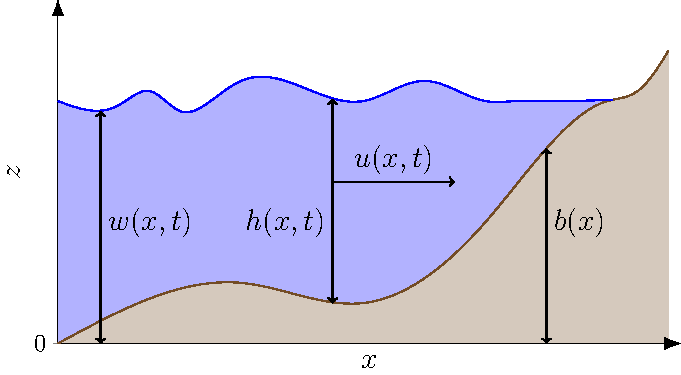
\includegraphics[width=0.7\textwidth]{./Figures/Diagrams/Watermodel/SerreModel.pdf}
	\caption{Diagram demonstrating a free surface flow (\squareF{blue}) over a bed (\squareF{brown!80!black}) where $w(x,t)$ is the absolute location of the free surface, $h(x,t)$ is the height of a column of fluid, $u(x,t)$ is the horizontal velocity of a column of fluid and $b(x)$ is the stationary bed profile.}
	\label{fig:SerreModel}
\end{figure}

\subsection{Conservation Law Form}

\begin{subequations}
	\label{eqn:FullSerreCon}
	\begin{align}
	& \frac{\partial h}{\partial t} + \dfrac{\partial (uh)}{\partial x} = 0 ,\label{eqn:FullSerreConMass}  \\ \nonumber \\
	\begin{split}
	\label{eqn:Serreconsconmom}
	\frac{\partial G}{\partial t}  + \frac{\partial}{\partial x} \left( {u} G + \frac{gh^2}{2} - \frac{2}{3}h^3 \left[\frac{\partial {u}}{\partial x}\right]^2 + h^2 {u}\frac{\partial {u}}{\partial x}\frac{\partial b}{\partial x} \right) \\ \\ +  \underbrace{\frac{1}{2}h^2 {u} \frac{\partial {u}}{\partial x} \frac{\partial^2 b}{\partial x^2}  - h {u}^2\frac{\partial b}{\partial x}\frac{\partial^2 b}{\partial x^2} + gh\frac{\partial b}{\partial x} } _{\text{source term}} = 0
	\end{split}
	\end{align}
\end{subequations}
with
\begin{equation}
\label{defn:SerreEqnConservedQuantity1}
G =  {u}h \left(1 + \frac{\partial h}{\partial x}\frac{\partial b}{\partial x} + \frac{1}{2}h\frac{\partial^2 b}{\partial x^2} + \left[\frac{\partial b}{\partial x}\right]^2 \right) - \frac{\partial}{\partial x}\left(\frac{1}{3}h^3  \frac{\partial {u}}{\partial x}\right)
\end{equation}

\subsection{Conservation Properties}

The total amount of a quantity $q$ in a system occurring on the interval $[a,b]$ at time $t$ is
\begin{equation*}
\mathcal{C}_q(t) = \int_{a}^{b} q(x,t)\, dx.
\end{equation*}

A system is conservative for a given quantity $q$ if $\mathcal{C}_{q}(0) = \mathcal{C}_{q}(t)$ for all $t$. The Serre equations conserve mass ($h$), momentum ($uh$), $G$ and the energy
\begin{equation*}
\mathcal{H}(x,t) = \frac{1}{2} \left( gh\left(h + 2b\right) + hu^2  + \frac{h^3}{3} \left[\frac{\partial u}{\partial x}\right]^2 + u^2h\left[\frac{\partial b}{\partial x}\right]^2 - uh^2 \frac{\partial u}{\partial x} \frac{\partial b}{\partial x}  \right).
\label{eqn:Hamildef}
\end{equation*}
The conservation of $h$, $uh$, $G$ is a result of integrating the Serre equations in conservative law form, and in their non-conservative form []. While the conservation of the energy $\mathcal{H}(x,t)$ is given by the derivation of the the Green-Naghdi equations \cite{Green-Naghdi-1976-237} which are equivalent to the Serre equations for one-dimensional flows. Indeed $\mathcal{H}$ is just a sum of the gravitational and kinetic energy throughout the depth of water. 

%--------------------------------------------------------------------------------
\section{Method}
%Brief overview
\begin{itemize}
	\item Reconstruction
	\item Finite Element Method
	\item Finite Volume Update
	\item Source Term
\end{itemize}

\subsection{Reconstruction}

\subsubsection{$h$, $w$ and $G$ }
We reconstruct $h$, $w$ and $G$ with piecewise linear functions over a cell from neighbouring cell averages. Since $h$, $w$ and $G$ use the same reconstruction operators we demonstrate them for a general quantity $q$. For the $j^{th}$ cell we reconstruct the values of $q$ at $x_{j-1/2} $, $x_{j} $ and $x_{j+1/2}$ in the following way
%cite someone 
\begin{subequations}
	\begin{align}
	q^+_{j-1/2} & = \mathcal{R}^+_{j-1/2} \left(\overline{\vecn{q}}\right) = \overline{q}_j - \dfrac{\Delta x}{2} d_j, \\
	q_{j} &= \mathcal{R}_{j} \left(\overline{\vecn{q}}\right) =\overline{q}_j ,\\
	q^-_{j+1/2} &= \mathcal{R}^-_{j+1/2} \left(\overline{\vecn{q}}\right) = \overline{q}_j + \dfrac{\Delta x}{2} d_j
	\end{align}
	\label{eqn:ReconforhwG}
\end{subequations}
where 
\begin{equation}
d_j = \text{minmod}\left(\theta \dfrac{\overline{q}_j -\overline{q}_{j-1} }{\Delta x}, \dfrac{\overline{q}_{j+1} -\overline{q}_{j-1} }{2\Delta x}, \theta\dfrac{\overline{q}_{j+1} -\overline{q}_{j} }{\Delta x}\right)
\label{eqn:slopehGrecon}
\end{equation}
with $\theta \in \left[1,2\right]$.

\subsubsection{Bed Profile}
For the bed profile we require a reconstruction that is at least second-order accurate for $b$, $\partial b / \partial x$ and $\partial^2 b / \partial x^2$. To accomplish this $b$ is reconstructed with a cubic polynomial $C_j(x)$ centred around $x_j$
\begin{equation*}
C_j(x) = c_0 \left(x - x_j\right)^3 + c_1 \left(x - x_j\right)^2 + c_2 \left(x - x_j\right) + c_3.
\label{eqn:cubicforbedrecon}
\end{equation*}

This cubic has the coefficients
\begin{align*}
&c_0 =  \dfrac{-b_{j-2} + 2b_{j-1} - 2 b_{j+1} + b_{j+2}}{12 \Delta x^3}, & &
c_1 =  \dfrac{b_{j-2} - b_{j-1} - b_{j+1} + b_{j+2}}{6 \Delta x^2},\\ \\
&c_2 =  \dfrac{b_{j-2} - 8b_{j-1} + 8 b_{j+1} - b_{j+2}}{12 \Delta x},& &
c_3 =  \dfrac{-b_{j-2}  + 4b_{j-1} + 4 b_{j+1} - b_{j+2}}{6}.
\end{align*}
We require a continuous bed profile and so we average the two reconstructions at the cell edge from the adjacent cells. Therefore, our reconstruction of the bed profile in the $j^{th}$ cell is the cubic which takes these values
\begin{subequations}
	\begin{align}
	b_{j-1/2} &=  \mathcal{B}_{j-1/2}\left(\vecn{b}\right) =  \frac{1}{2}\left( C_j(x_{j-1/2}) + C_{j-1}(x_{j-1/2})\right),\\
	b_{j-1/6} &=  \mathcal{B}_{j-1/6}\left(\vecn{b}\right) =  C_j(x_{j-1/6}),\\
	b_{j+1/6} &=  \mathcal{B}_{j+1/6}\left(\vecn{b}\right) =  C_j(x_{j+1/6}),\\
	b_{j+1/2} &=  \mathcal{B}_{j+1/2}\left(\vecn{b}\right) =  \frac{1}{2}\left( C_j(x_{j+1/2}) + C_{j+1}(x_{j+1/2})\right).
	\end{align}
	\label{eqn:BedReconDef}
\end{subequations}

\subsection{Velocity Solve using a Finite Element Method}
In the FEVM we solve for the primitive variable $u$ given $h$, $G$ and $b$ using a finite element approximation to \eqref{defn:SerreEqnConservedQuantity1}. For the FEM we begin with the weak form of \eqref{defn:SerreEqnConservedQuantity1} using test function $v$ over the spatial domain $\Omega$ which is 

\begin{equation*}
\int_{\Omega } G v \; dx =  \int_{\Omega } uh \left(1 + \frac{\partial h}{\partial x}\frac{\partial b}{\partial x} + \frac{1}{2}h\frac{\partial^2 b}{\partial x^2} +  \left[\frac{\partial b}{\partial x}\right]^2 \right) v - \frac{\partial}{\partial x}\left(\frac{1}{3}h^3  \frac{\partial {u}}{\partial x}\right) v \; dx.
\end{equation*}

Integrating by parts with zero Dirichlet boundary conditions we get
\begin{multline}
\int_{\Omega } G v \; dx = \int_{\Omega } uh \left(1 + \left[\frac{\partial b}{\partial x}\right]^2 \right) v \; dx +  \int_{\Omega } \frac{1}{3}h^3  \frac{\partial {u}}{\partial x} \frac{\partial v}{\partial x} \; dx  \\ - 
\int_{\Omega }   \frac{1}{2} u h^2\frac{\partial b}{\partial x}  \frac{\partial v }{\partial x}\; dx - 
\int_{\Omega }   \frac{1}{2}h^2\frac{\partial b}{\partial x}  \frac{\partial u }{\partial x}v \; dx.
\label{eqn:WeakFormDomain}
\end{multline}
By assuming that time is fixed so that all the functions only vary in space, this formulation implies that by ensuring that $G$, $h$, $b$ and $\partial b / \partial x$ have finite integrals over $\Omega$, then $u$ and $\partial u / \partial x$ must have finite integrals as well. Since we require $\partial u / \partial x$ to be well defined to approximate the flux and the source terms \eqref{eqn:FullSerreCon} and thus have finite integrals we will assume that for each time $t$ that $h,G \in \mathbb{L}^2(\Omega)$ and $b \in\mathbb{W}^{1,2}(\Omega)$ so that $u \in \mathbb{W}^{1,2}(\Omega)$. See Appendix \ref{app:FEMIntegrals} for a precise definition of $\mathbb{L}^2(\Omega)$ and $\mathbb{W}^{1,2}(\Omega)$.

We simplify \eqref{eqn:WeakFormDomain} by performing the integration over the cells and then summing the integrals together to get the equation for the entire domain
\begin{multline}
\label{eq:elementwiseint}
\sum_{j=0}^m \Bigg(  \int_{x_{j-1/2} }^{{x_{j+1/2}}} \Bigg[  \left( uh \left(1 + \left[\frac{\partial b}{\partial x}\right]^2 \right)  - \frac{1}{2}h^2\frac{\partial b}{\partial x}  \frac{\partial u }{\partial x}  -  G \right) v   \\ +  \left(\frac{1}{3}h^3  \frac{\partial {u}}{\partial x}    -     \frac{1}{2} uh^2\frac{\partial b}{\partial x}    \right) \frac{\partial v }{\partial x} \Bigg]dx \Bigg)  = 0
\end{multline}
which holds for all test functions $v$. The next step is to replace the functions for $h$, $G$, $b$, $v$ and $u$ with their corresponding basis function approximations.

For $h$ and $G$ we use the basis functions $\psi$ \eqref{eqn:App1:PsiDef} which are linear inside a cell and zero elsewhere and so are not continuous as shown in Figure \ref{fig:P1DiscBasis}. This is consistent with our reconstruction which is second-order accurate inside the cell and possesses discontinuities at the cell edges. Since these basis functions are in $\mathbb{L}^2(\Omega)$ our basis function approximations to $h$ and $G$ are in the appropriate function space.
\begin{figure}
	\centering
		\begin{subfigure}{0.45\textwidth}
			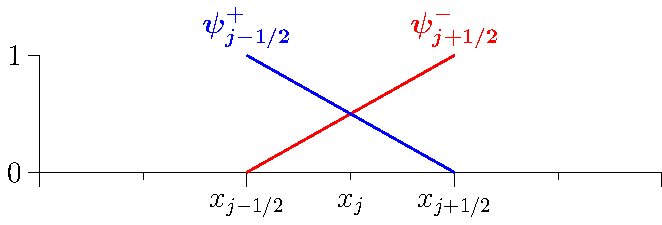
\includegraphics[width=\textwidth]{./Figures/Diagrams/FEMbasis/P1/P1NN-figure0.pdf}
			\subcaption{$\psi$}
			\vspace{0.5cm}
		\end{subfigure}
		\begin{subfigure}{0.45\textwidth}
			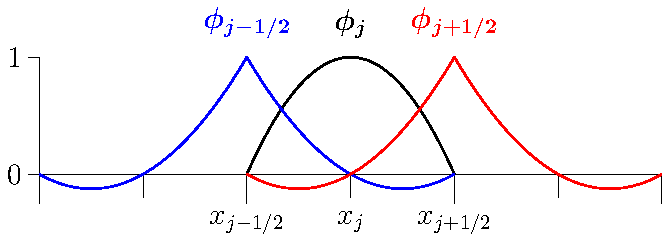
\includegraphics[width=\textwidth]{./Figures/Diagrams/FEMbasis/P2/P2N-figure0.pdf}
			\subcaption{$\phi$}
			\vspace{0.5cm}
		\end{subfigure}
		\begin{subfigure}{0.6\textwidth}
			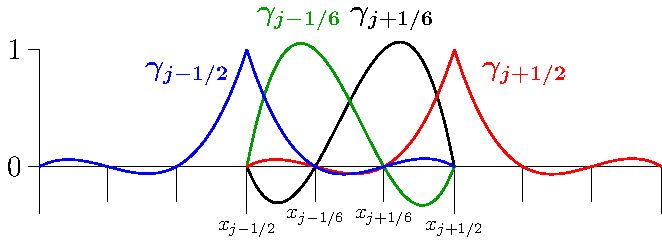
\includegraphics[width=\textwidth]{./Figures/Diagrams/FEMbasis/P3/P3-figure0.pdf}
			\subcaption{$\gamma$}
			\vspace{0.5cm}
		\end{subfigure}
	\caption{Support of the basis functions $\psi$, $\phi$ and $\gamma$ which are non-zero over the $j^{th}$ cell.}
	\label{fig:P1DiscBasis}
\end{figure}

From the basis functions $\psi$ we have the following representation for $h$ and $G$ in our FEM written for the generic quantity $q$
\begin{align}
\label{eqn:FEapproxtohG}
q &= \sum_{j=0}^m \left( q^+_{j-1/2}\psi^+_{j-1/2}  + q^-_{j+1/2}\psi^-_{j+1/2}, \right).
\end{align}
For $u$ we use
\begin{equation}
u = u_{-1/2}\phi_{-1/2} + \sum_{j=0}^m \left( u_{j}\phi_{j} + u_{j+1/2}\phi_{j+1/2} \right).
\label{eqn:FEapproxtou}
\end{equation}
While for $b$ we use
\begin{equation}
b = b_{-1/2}\gamma_{-1/2} +  \sum_{j=0}^m \left(b_{j-1/6}\gamma_{j-1/6}  + b_{j+1/6}\gamma_{j+1/6} + b_{j+1/2}\gamma_{j+1/2} \right).
\label{eqn:FEapproxtob}
\end{equation}

By combining all the matrices generated by the integral of each of the $u$ terms we get the contribution of the $j^{th}$ cell to the stiffness matrix $\matr{A}_j$. Likewise all the integrals of the remaining term $Gv$ in \eqref{eq:elementwiseint} generate the element wise vector $\vecn{g}_{j}$. These element wise matrices and vectors are then assembled into the global stiffness matrix $\matr{A}$ and the global right hand-side term $\vecn{g}$ thus \eqref{eq:elementwiseint} is rewritten as
\begin{equation}
\label{eqn:FEMElemMatrixJ}
\matr{A} \vecn{\hat{u}} = \vecn{g}.
\end{equation}
This is a penta-diagonal matrix equation which can be solved by direct banded matrix solution techniques such as those of \citet{NumRecC-1996} to obtain
\begin{equation}
\vecn{\hat{u}} =\mathcal{G}\left( \vecn{\hat{h}}, \vecn{\hat{G}},\vecn{\hat{b}} \right) =   \matr{A}^{-1}\vecn{g}
\label{eqn:usolvefromGhb}
\end{equation}
as desired.

\subsection{Flux Approximation}
We use the method of \citet{Kurganov-etal-2001-707} to calculate the flux across a cell interface. This method was employed because it can handle discontinuities across the cell boundary and only requires an estimate of the maximum and minimum wave speeds. This is precisely the situation for the Serre equations which do not have a known expression for the characteristics but do possess estimates on the maximum and minimum wave speeds \eqref{eqn:WaveVelocitiesBound}.

Only the calculation of the flux term $F_{j+1/2}$ is demonstrated as the process to calculate the flux term $F_{j-1/2}$ is identical but with different cells. For a general quantity $q$ the approximation of the flux term given by \citet{Kurganov-etal-2001-707} is
\begin{equation}\label{eqn:HLL_flux}
F_{j+\frac{1}{2}} = \dfrac{a^+_{j+\frac{1}{2}} f\left(q^-_{j+\frac{1}{2}}\right) - a^-_{j+\frac{1}{2}} f\left(q^+_{j+\frac{1}{2}}\right)}{a^+_{j+\frac{1}{2}} - a^-_{j+\frac{1}{2}}}  + \dfrac{a^+_{j+\frac{1}{2}} \, a^-_{j+\frac{1}{2}}}{a^+_{j+\frac{1}{2}} - a^-_{j+\frac{1}{2}}} \left(  q^+_{j+\frac{1}{2}} - q^-_{j+\frac{1}{2}} \right)
\end{equation}
where $a^+_{j+\frac{1}{2}}$ and $a^-_{j+\frac{1}{2}}$ are given by bounds on the wave speed. Applying the wave speed bounds \eqref{eqn:WaveVelocitiesBound} we obtain

\begin{align}
a^-_{j+\frac{1}{2}} &= \min\left\lbrace 0\;,\;  u^-_{j + 1/2} - \sqrt{g h^-_{j + 1/2}}  \;,\;u^+_{j + 1/2} - \sqrt{g h^+_{j + 1/2}} \right\rbrace  ,\\
a^+_{j+\frac{1}{2}} &= \max\left\lbrace 0 \;,\;  u^-_{j + 1/2} + \sqrt{g h^-_{j + 1/2}}  \;,\;u^+_{j + 1/2} + \sqrt{g h^+_{j + 1/2}} \right\rbrace .
\label{eqn:WaveSpeedBoundsFluxApprox}
\end{align}

To recover the lake at rest steady state solution we follow the work of \citet{Klein-etal-2004-2050}, who accomplished this for the SWWE. Previously, we demonstrated that this process can be extended to the Serre equations \cite{Pitt-J-2014}. To enforce well-balancing the reconstruction of $h$ is modified at the cell edges in the following way.

First calculate
\begin{align}
\dot{b}^-_{j+1/2} = w^-_{j+1/2} - h^-_{j+1/2} &, &\dot{b}^+_{j+1/2} = w^+_{j+1/2} - h^+_{j+1/2}.
\label{eqn:BedReDefWmH}
\end{align}
Find the maximum
\begin{align*}
\ddot{b}_{j+1/2} = \max\left\lbrace\dot{b}^-_{j+1/2} , \dot{b}^+_{j+1/2} \right\rbrace
\end{align*}
then define
\begin{subequations}
	\begin{align}
	\ddot{h}^-_{j+1/2} &= \max\left\lbrace 0, w^-_{j+1/2} - \ddot{b}_{j+1/2}  \right\rbrace, \\  \ddot{h}^+_{j+1/2} &= \max\left\lbrace 0, w^+_{j+1/2} - \ddot{b}_{j+1/2} \right\rbrace.
	\end{align}
	\label{eqn:ModifiedHValue}
\end{subequations}
This generates the vector $\vecn{\ddot{h}}$
\begin{equation*}
\vecn{\ddot{h}}= \begin{bmatrix} \TM
\ddot{h}^+_{-1/2} \\ h_0 \\ \ddot{h}^-_{1/2} \\ \vdots  \\ \ddot{h}^-_{m + 1/2}  \BM \end{bmatrix}
\end{equation*}
which we use to calculate the flux term $F_{j+1/2}$ in \eqref{eqn:HLL_flux} for $h$ and $G$ instead of $\vecn{\hat{h}}$. Applying the same process but with different cells we obtain $F_{j-1/2}$ and we have
\begin{align*}	
F^n_{j\pm 1/2} &=\mathcal{F}_{j\pm1/2} \left(\vecn{\ddot{h}}, \vecn{\hat{G}},\vecn{\hat{b}}, \vecn{\hat{u}}  \right).
\end{align*}
for the evolution of $h$ and $G$ equations as desired.

The flux functions $f(q^-_{j+\frac{1}{2}})$ and $f(q^+_{j+\frac{1}{2}})$ across the cell edge $x_{j+1/2}$ are evaluated using the reconstructed values $q^-_{j+\frac{1}{2}}$ from the $j^{th}$ cell and $q^+_{j+\frac{1}{2}}$ from the $(j+1)^{th}$ cell. From the continuity equation \eqref{eqn:FullSerreConMass} we have
\begin{align*}
f\left(h^\pm_{j+\frac{1}{2}}\right) &= u^\pm_{j + 1/2}  h^\pm_{j + 1/2}.
\end{align*}

For the evolution of $G$ equation \eqref{eqn:Serreconsconmom} we have 
\begin{align}
f\left(G^\pm_{j+\frac{1}{2}}\right) &=  u^\pm_{j + 1/2} G^\pm_{j + 1/2}  + \frac{g}{2}\left(h^\pm_{j + 1/2} \right)^2 - \frac{2}{3}\left(h^\pm_{j + 1/2}\right)^3 \left[\left(\frac{\partial {u}}{\partial x} \right)^\pm_{j + 1/2} \right]^2 \nonumber\\ &+ \left(h^\pm_{j + 1/2}\right)^2 u^\pm_{j + 1/2} \left(\frac{\partial {u}}{\partial x} \right)^\pm_{j + 1/2} \left(\frac{\partial b}{\partial x} \right)^\pm_{j + 1/2} .
\label{eqn:FluxIrrotNum}
\end{align}

The quantities $h^+_{j - 1/2}$, $h^-_{j + 1/2}$, $G^+_{j - 1/2}$ and $G^-_{j + 1/2}$ were calculated during the reconstruction and the FEM provided $u^\pm_{j+1/2} = u_{j+1/2}$ as $u$ is continuous across the cell boundaries.

For $P^u_j(x)$ we obtain the coefficients
\begin{align*}
p^u_0 &=  \dfrac{u_{j-1/2} - 2u_j + u_{j+1/2}}{2 \Delta x^2},\\
p^u_1 &=  \dfrac{-u_{j-1/2} + u_{j+1/2}}{\Delta x},\\
p^u_2 &=  u_j.
\end{align*}
While for $P^b_j(x)$ the coefficients are
\begin{align*}
p^b_0 &=  \dfrac{-9b_{j-1/2} + 27b_{j-1/6} - 27 b_{j+1/6} + 9b_{j+1/2}}{2 \Delta x^3},\\ \\
p^b_0 &=  \dfrac{9b_{j-1/2} - 9b_{j-1/6} - 9b_{j+1/6} + 9b_{j+1/2}}{4 \Delta x^2},\\ \\ 
p^b_0 &=  \dfrac{b_{j-1/2} - 27b_{j-1/6} + 27 b_{j+1/6} - b_{j+1/2}}{8 \Delta x},\\\\
p^b_0 &=  \dfrac{-b_{j-1/2}  + 9b_{j-1/6} + 9 b_{j+1/6} - b_{j+1/2}}{16}.
\end{align*}
Taking the derivative of the polynomials \eqref{eqn:Polyforucell} and \eqref{eqn:Polyforbcell} we get
\begin{align*}
\frac{\partial }{\partial x}P^u_j(x) &= 2p^u_0 \left(x - x_j\right) + p^u_1, \\
\frac{\partial }{\partial x}P^b_j(x) &= 3p^b_0 \left(x - x_j\right)^2 + 2p^b_1 \left(x - x_j\right) + p^b_2.
\end{align*}
This gives a second-order approximation to the derivative of $u$ and $b$ at $x_{j+1/2}$ for the $j^{th}$ cell. The process for the $(j+1)^{th}$ cell is the same and we get 
\begin{align*}
\left(\dfrac{\partial {u}}{\partial x} \right)^-_{j + 1/2} &= \frac{\partial }{\partial x}P^u_j(x_{j+1/2}),  \\
\left(\dfrac{\partial {u}}{\partial x} \right)^+_{j + 1/2} &= \frac{\partial }{\partial x}P^u_{j+1}(x_{j+1/2}),  \\
\left(\dfrac{\partial {b}}{\partial x} \right)^-_{j + 1/2} &= \frac{\partial }{\partial x}P^b_j(x_{j+1/2}), \\
\left(\dfrac{\partial {b}}{\partial x} \right)^+_{j + 1/2} &= \frac{\partial }{\partial x}P^b_{j+1}(x_{j+1/2}). 	\end{align*}

\subsection{Source Term Approximation}

To evolve the Serre equations \eqref{eqn:FullSerreCon}, we require an approximation to the source term at the cell centre $x_j$ from time $t^n$ to $t^{n+1}$ which we denote as $S^n_j$. Equation \eqref{eqn:FullSerreConMass} has no source term, therefore we only present the calculation of the source term for equation \eqref{eqn:Serreconsconmom}.

Following the work of \citet{Klein-etal-2004-2050} to produce a well-balanced method, we split our approximation to $S^n_j$ into the centred source term $S_{ci}$ and the corrective interface source terms $S^{-}_{j + \frac{1}{2}}$ and $S^{+}_{j + \frac{1}{2}}$
\begin{equation*}
S^n_j =  S^{-}_{j + \frac{1}{2}} + \Delta x S_{ci} + S^{+}_{j - \frac{1}{2}}.
\end{equation*}
Where $S_{ci}$ is the naive source term approximation and $S^{-}_{j + \frac{1}{2}}$ and $S^{+}_{j + \frac{1}{2}}$ are correction terms that ensure that the flux and source term cancel for the lake at rest solution. 

We calculate the centred source term using
\begin{equation*}
S_{ci} = -\frac{1}{2}\left(h_j\right)^2 {u_j}\left( \frac{\partial {u}}{\partial x} \right)_j \left(\frac{\partial^2 b}{\partial x^2} \right)_j  + h_j \left(u_j\right)^2 \left(\frac{\partial b}{\partial x}\right)_j \left(\frac{\partial^2 b}{\partial x^2}\right)_j - gh_j\left(\frac{\partial b}{\partial x}\right)_j.
\end{equation*}
Where we use $h_j$ from the reconstruction process \eqref{eqn:ReconforhwG} and $u_j$ from the solution of \eqref{eqn:usolvefromGhb}. To calculate the derivatives we employ our polynomial representations of $u$ \eqref{eqn:Polyforucell} and $b$ \eqref{eqn:Polyforbcell} inside a cell. However, to ensure that the terms cancel properly for a lake at rest we modify our approximation to $\dfrac{\partial b}{\partial x}$ to use $\dot{b}^-_{j+1/2}$ and $\dot{b}^+_{j+1/2}$ from \eqref{eqn:BedReDefWmH}. Therefore, the following approximations are used to calculate $S_{ci}$
\begin{align*}
\left(\dfrac{\partial {u}}{\partial x} \right)_{j} &= \frac{\partial }{\partial x}P^u_j(x_{j}),  \\
\left(\dfrac{\partial {b}}{\partial x} \right)_{j} &=  \frac{\dot{b}^-_{j+1/2} - \dot{b}^+_{j-1/2}}{\Delta x} , \\	
\left(\dfrac{\partial^2 {b}}{\partial x^2} \right)_{j} &= \frac{\partial^2 }{\partial x^2}P^b_j(x_{j}).
\end{align*}

To ensure well-balancing the corrective interface source terms
\begin{align*}
S^{-}_{j + \frac{1}{2}} &=  \frac{g}{2} \left(\ddot{h}^{-}_{j + \frac{1}{2}} \right)^2 - \frac{g}{2} \left(h^{-}_{j + \frac{1}{2}} \right)^2, \\ \\
S^{+}_{j - \frac{1}{2}} &=  \frac{g}{2} \left(h^{+}_{j - \frac{1}{2}}\right)^2 - \frac{g}{2}\left(\ddot{h}^{+}_{j - \frac{1}{2}}\right)^2 
\end{align*}
are also added. These corrective terms make use of $h^{-}_{j + \frac{1}{2}}$ and $h^{+}_{j + \frac{1}{2}}$ obtained from the reconstruction \eqref{eqn:ReconforhwG} and the modified values $\ddot{h}^{-}_{j + \frac{1}{2}}$ and $\ddot{h}^{+}_{j + \frac{1}{2}}$ from \eqref{eqn:ModifiedHValue}. Combining the centred and interface source terms our approximation to the source term for $G$ is 
\begin{equation*}
S^n_j = \mathcal{S}_j\left( \vecn{\hat{h}},\vecn{\ddot{h}},\vecn{\hat{w}},\vecn{\hat{b}}, \vecn{\hat{u}}  \right)=   S^{-}_{j + \frac{1}{2}} + \Delta x S_{ci} + S^{+}_{j - \frac{1}{2}}.
\end{equation*}
This operator $\mathcal{S}_j$ is slightly different to the example given in the overview of the evolution step as it takes $\vecn{\hat{h}}$ and $\vecn{\ddot{h}}$ as inputs. This change was made to make clear that $\vecn{\ddot{h}}$ is required to calculate $S^n_j$. This would be obscured by a more consistent notation that is possible since $\vecn{\ddot{h}}$ only depends on $\vecn{\hat{h}}$, $\vecn{\hat{w}}$ and $\vecn{\hat{b}}$. 

\subsection{Time-Stepping}

To increase the order of accuracy in time we employ the Strong Stability Preserving (SSP) Runge-Kutta method \cite{Gottlieb-etal-2003-89} which is a convex combination of the first-order time steps \eqref{eqn:UpdateMethod} in the following way
\begin{subequations}
	\begin{align}
	\overline{q}_j^{(1)} &= \overline{q}^{n}_j + \frac{\Delta t}{\Delta x} \left(F^n_{j+\frac{1}{2}} - F^n_{j-\frac{1}{2}} + S^n_j\right),\\
	\overline{q}_j^{(2)} &= \overline{q}_j^{(1)} + \frac{\Delta t}{\Delta x} \left(F_{j+\frac{1}{2}}^{(1)} - F_{j-\frac{1}{2}}^{(1)}  + S_j^{(1)} \right), \\
	\overline{q}^{n+1}_j &= \frac{1}{2} \left( \overline{q}^n_j +  \overline{q}_j^{(2)}  \right).
	\end{align}
	\label{eqn:SSPRKStep1}
\end{subequations}
%TVD no oscillations introduced by the particular method
This results in a time stepping method that preserves the stability of the first-order method \eqref{eqn:UpdateMethod} and is second-order accurate in time. Since all the spatial approximations are second-order accurate, the steps (i)-(vi) should result in a second-order accurate FEVM for the Serre equations, as desired. 


\subsection{Dry Bed Handling}

\begin{subequations}
	\begin{align}
	h^+_{j-1/2} & = h^+_{j-1/2} \left(\frac{ h^+_{j-1/2}  + h_{base}}{h^+_{j-1/2} + h_{tol}}\right) , \\ \nonumber\\
	h^-_{j+1/2} & = h^-_{j+1/2} \left(\frac{ h^-_{j+1/2}  + h_{base}}{h^-_{j+1/2} + h_{tol}}\right)
	\end{align} 
	\label{eqn:hdrytransform}
\end{subequations}

%----------
\section{Lake at Rest Solution Validation}

\begin{subequations}
	\begin{align}
	&h(x,t) = \max\left\lbrace a_0 - b(x), 0 \right\rbrace, & b(x) = a_1 \sin\left(a_2 x\right), \\
	&u(x,t) = 0 , 	&G(x,t) = 0 .
	\end{align}
	\label{eqn:LARdefhub}
\end{subequations}
was chosen for this validation to ensure that all terms with derivatives of the bed were tested. To demonstrate the capability of the methods in the presence of dry and wet beds the parameter values $a_0 = 0m$, $a_1 = 1m$ and $a_2 = 2 \pi / 50 m^{-1} $ were chosen. These parameter values result in wet regions with a horizontal free surface where the stage $w(x,t)= h(x,t) + b(x) =a_0= 0$ \eqref{eqn:LARdefhub}. Therefore, we have a periodic bed where water submerges the troughs of the bed while the peaks of the bed are dry. 

For the numerical solutions the spatial domain was $x \in \left[-112.5 m,87.5 m\right]$ and the final time was $t=10s$, with the standard gravitational acceleration $g= 9.81 m/s^2$. The spatial resolution of the method was varied so that $\Delta x = 100 / 2^k m$ with $k \in \left[8, \dots ,17\right]$ and the CFL condition \eqref{eqn:CFLcond} was satisfied by having $\Delta t = Cr \Delta x / \sqrt{g}$ with condition number $Cr = 0.5$. The standard limiting parameter $\theta = 1.2$ was used in the generalised minmod limiter, \eqref{eqn:slopehGrecon} for both $\text{FEVM}_2$ and $\text{FDVM}_2$. Dirichlet boundary conditions were used at both ends as the analytic solution is stationary.

The numerical methods are assessed by using the specified lake at rest solution as initial conditions and comparing the numerical solutions of $\text{FEVM}_2$ and $\text{FDVM}_2$ at $t=10s$ to the analytic solution, which are the initial conditions. To demonstrate the utility of the well-balancing method the results from two versions of $\text{FEVM}_2$ and $\text{FDVM}_2$ are presented, where the well-balancing method described in Chapter \ref{chp:HFVMMethod} is and is not employed. 

Example numerical solutions with $\Delta x = 100/2^{10}m \approx 0.0977m$ at $t=10s$ for all versions of $\text{FEVM}_2$ and $\text{FDVM}_2$ are given in Figure \ref{fig:LakeAtRestEx}. The numerical solutions in these figures are indistinguishable from the analytic solutions at this scale and so the analytic solutions have been omitted from the plots. 


\begin{figure}
	\centering
		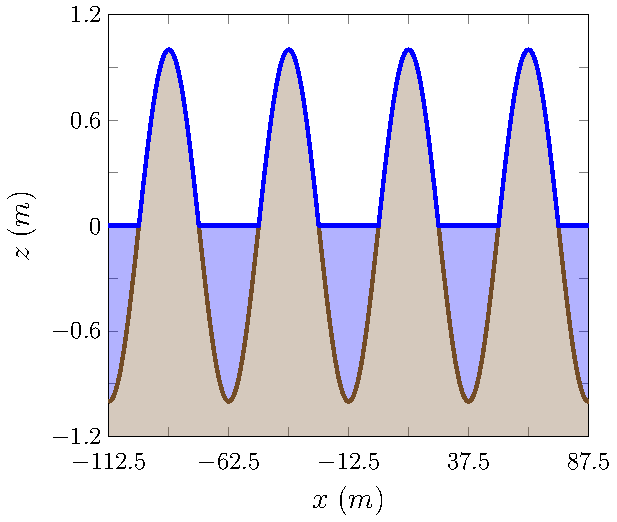
\includegraphics[width=0.7\textwidth]{./Figures/LakeAtRest/Exw.pdf}
	\caption{Numerical solution for $w$ (\squareF{blue}) and $b$ (\squareF{brown!60!black}) with $\Delta x = {100} / {2^{10}}m $ for the lake at rest problem at $t=10s$.}
	\label{fig:LAR}
\end{figure}
\begin{figure}
	\centering
	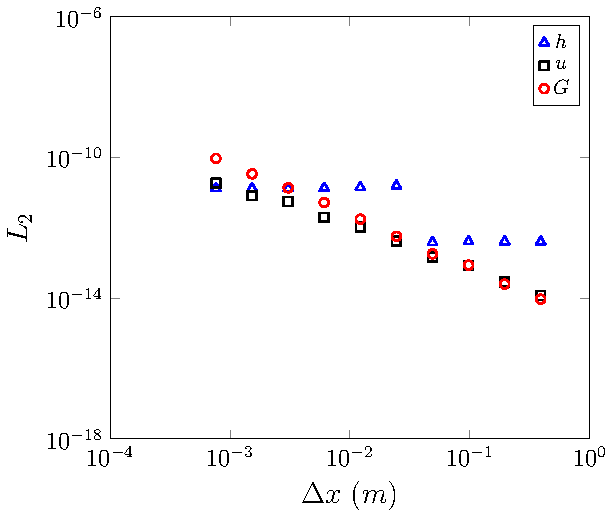
\includegraphics[width=0.7\textwidth]{./Figures/LakeAtRest/L2.pdf}
	\caption{Convergence as measured by the $L_2$ norm against $\Delta x$ for $h$ , $u$ and $G$ for the lake at rest problem at $t=10s$.}
	\label{fig:LARL1}
\end{figure}
\begin{figure}
	\centering
		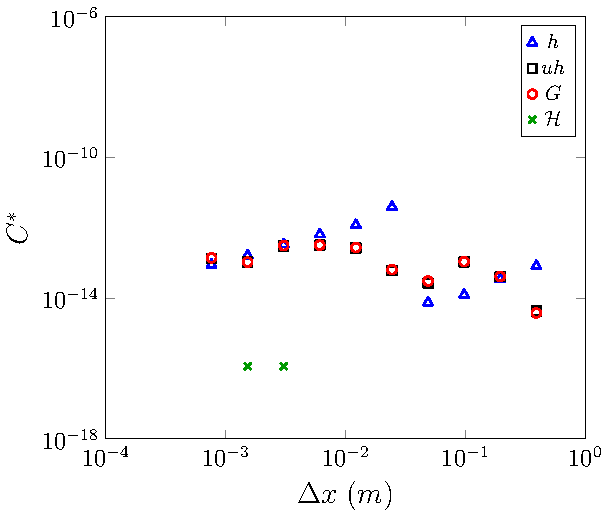
\includegraphics[width=0.7\textwidth]{./Figures/LakeAtRest/C1num.pdf}
		\subcaption{numerical conservation error}
		\vspace{0.5cm}
	\caption{Conservation error against $\Delta x$ for $h$, $u$, $G$ and $\mathcal{H}$ for the lake at rest problem at $t=10s$.}
	\label{fig:LarC}
\end{figure}

%--------------------------------------------------------------------------------
\section{Forced Solution Validation}


	
\subsection{Forced Solution}

The known analytic solutions of the Serre equations provide a stringent test when the bed is horizontal, as all terms in the equations are non-zero and vary in space and time. For varying bathymetry there is only the lake at rest solution where all terms are constant in time and some vanish. Therefore, the accuracy of the approximations of all terms of the Serre equations in the numerical method is not adequately assessed using only the currently available analytic solutions.

Currently the verification of the order of accuracy of the numerical methods for transient solutions with varying bathymetry requires the use of forced solutions. To do this we select some particular functions for all of the primitive quantities; $h$, $u$ and $b$ which we denote $h^*$, $u^*$ and $b^*$ respectively. To force these functions $h^*$, $u^*$ and $b^*$ to be solutions of the Serre equations \eqref{eqn:FullSerreCon} we add the terms $S_h$ and $S_G$ to obtain the forced Serre equations
\begin{subequations}
	\label{eqn:FullSerreConForced}
	\begin{align}
	& \frac{\partial h}{\partial t} + \dfrac{\partial (uh)}{\partial x} + S_{h}  = 0 ,\label{eqn:FullSerreConMassForced}  \\ \nonumber \\
	\begin{split}
	\label{eqn:SerreconsconmomForced}
	\frac{\partial G}{\partial t}  + \frac{\partial}{\partial x} \left( {u} G + \frac{gh^2}{2} - \frac{2}{3}h^3 \left[ \frac{\partial {u}}{\partial x} \right]^2 + h^2 {u}\frac{\partial {u}}{\partial x}\frac{\partial b}{\partial x} \right) \\ \\ + \frac{1}{2}h^2 {u} \frac{\partial {u}}{\partial x} \frac{\partial^2 b}{\partial x^2}  - h {u}^2\frac{\partial b}{\partial x}\frac{\partial^2 b}{\partial x^2} + gh\frac{\partial b}{\partial x} + S_{G} = 0
	\end{split}
	\end{align}
\end{subequations}
where
\begin{align*}
&  S_{h} = -\frac{\partial h^*}{\partial t} - \dfrac{\partial (u^*h^*)}{\partial x} ,  \\ \nonumber \\
\begin{split}
S_{G} = -\frac{\partial G^*}{\partial t}  - \frac{\partial}{\partial x} \left( {u}^* G^* + \frac{g\left[h^*\right]^2}{2} - \frac{2}{3}\left[h^*\right]^3 \left[\frac{\partial {u}^*}{\partial x}\right]^2 + \left[h^*\right]^2 {u^*}\frac{\partial {u}^*}{\partial x}\frac{\partial b^*}{\partial x} \right) \\ \\ - \frac{1}{2}\left[h^*\right]^2 {u}^* \frac{\partial {u}^*}{\partial x} \frac{\partial^2 b^*}{\partial x^2}  + h^* {\left[u^*\right]}^2\frac{\partial b^*}{\partial x}\frac{\partial^2 b^*}{\partial x^2} - gh^*\frac{\partial b^*}{\partial x}.
\end{split}
\end{align*} 
These forced Serre equations are then numerically solved by solving the Serre equations \eqref{eqn:FullSerreCon} with the analytic values of $S_{h}$ and $S_{G}$ given $h^*$, $u^*$ and $b^*$. So that, the only error present in the numerical solutions of the forced Serre equations is the error produced by the numerical methods used to solve the Serre equations.

Note that since the choice of the forced solutions $h^*$, $u^*$ and $b^*$ is arbitrary the solutions of the forced Serre equations need not be conservative or retain any properties of the underlying Serre equations. 

\subsection{Dry Bed Forced Solution Problem}

\begin{subequations}
	\begin{align}
	\label{eqn:ForcedSolutionxt}
	h^*(x,t) &= a_0 + a_1 \exp\left(-\dfrac{\left[\left(x - a_2 t\right) - a_3\right]^2}{2 a_4}\right), \\
	u^*(x,t) &= a_5 \exp\left(-\dfrac{\left[\left(x - a_2 t\right) - a_3\right]^2}{2 a_4}\right), \\
	b^*(x) &= a_6 \sin\left(a_7 x\right)
	\end{align}
\end{subequations}
for the primitive variables were chosen. These functions produce an $a_1$ high Gaussian bump for $h$ and $u$ that travels at a fixed speed $a_2$ over a periodic bed. Thus, $h$ and $u$ will have constant shape and travel to the right over time. However, this is not the case for $G$ as $u$ and $h$ have constant shape but the bed is periodic. With the bed terms in $G$ \eqref{defn:SerreEqnConservedQuantity1} changing the shape of $G$ as the Gaussian bump in $h$ and $u$ encounters different bed slopes.

For non-trivial choices of the parameters $a_i$ all terms in the Serre equations vary in space and time and so all terms must be accurately approximated by the numerical method to adequately reproduce the forced solution. 

Both validation studies used the values $a_1 = 0.5m$, $a_2 = 2 \pi / \left(10 a_7\right) m/s$, $a_3 =- 3\pi/ \left(2 a_7\right)m$, $a_4 = \pi / (16 a_7) m^2$, $a_5 = 0.5 m/s$, $a_6 = 1.0 m$ and $a_7 = \pi / 25 m^{-1}$ with $a_0= 1m$ for the finite water depth forced solution and $a_0=0m$ for the dry bed forced solution. These parameter values result in a Gaussian bump in $h$ and $u$ that has a width much smaller than the wavelength of the bed profile and travels precisely one wavelength in $10s$.

The domain of the numerical solutions was $x \in \left[-112.5 m,87.5 m\right]$ with $t \in \left[0s,10s\right]$. The standard gravitational acceleration $g= 9.81 m/s^2$ was used. The spatial resolution of numerical methods was varied like so $\Delta x = 100 / 2^k m$ with $k \in \left[8,\dots,17\right]$. To satisfy the CFL condition, \eqref{eqn:CFLcond} the temporal resolution
$\Delta t = Cr \Delta x / \left(a_2 + a_5 + \sqrt{g\left(a_0 + a_1\right)}\right)$ was chosen with condition number $Cr = 0.5$. The value $\theta = 1.2$ was used in the generalised minmod limiter \eqref{eqn:slopehGrecon} for both $\text{FEVM}_2$ and $\text{FDVM}_2$ and Dirichlet boundary conditions were applied at the boundaries of the domain. 

\begin{figure}
	\centering
	\begin{subfigure}{0.5\textwidth}
		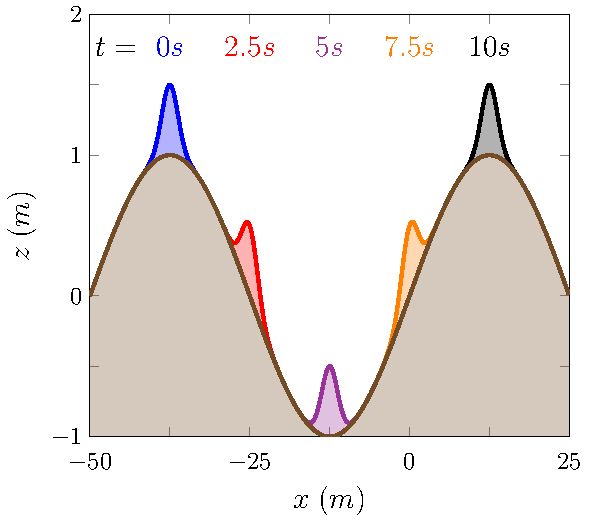
\includegraphics[width=\textwidth]{./Figures/Forced/Dry/w.pdf}
		\subcaption{$w$ and $b$ (\squareF{brown!60!black})}
		\vspace{0.5cm}
	\end{subfigure}%
	\begin{subfigure}{0.5\textwidth}
	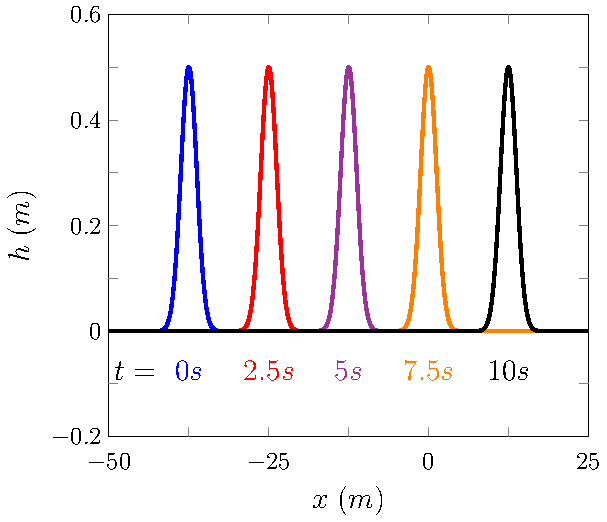
\includegraphics[width=\textwidth]{./Figures/Forced/Dry/h.pdf}
		\subcaption{$h$}
		\vspace{0.5cm}
	\end{subfigure}
	\begin{subfigure}{0.5\textwidth}
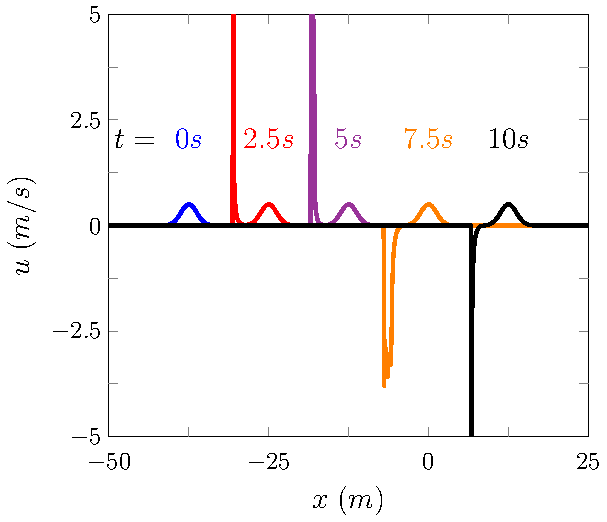
\includegraphics[width=\textwidth]{./Figures/Forced/Dry/u.pdf}
\subcaption{$u$}
		\vspace{0.5cm}
	\end{subfigure}%
	\begin{subfigure}{0.5\textwidth}
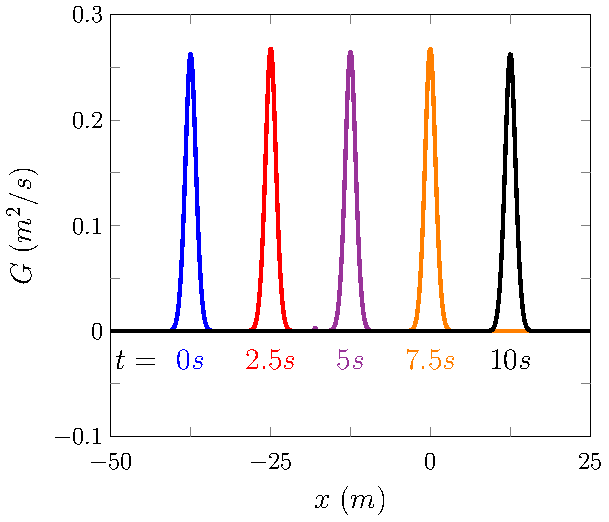
\includegraphics[width=\textwidth]{./Figures/Forced/Dry/G.pdf}
\subcaption{$G$}
		\vspace{0.5cm}
	\end{subfigure}
	\caption{Example numerical solutions for $w$, $b$, $h$, $G$ with $\Delta x = 100 / 2^{10}m$ at various times to the dry bed forced solution problem.}
	\label{fig:ExampleForcedSolutionDry}
\end{figure}

\begin{figure}
	\centering
		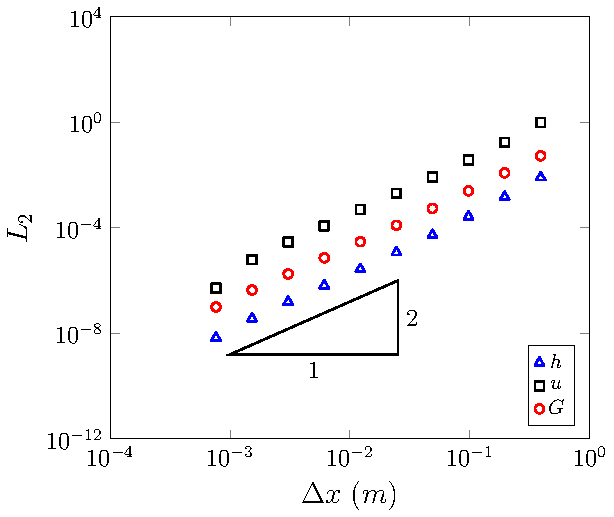
\includegraphics[width=0.7\textwidth]{./Figures/Forced/Dry/L2red.pdf}
	\caption{Convergence as measured by the $L_2$ in regions where $h > 10^{-3}m$ norm against $\Delta x$ for $h$, $u$, and $G$ for the dry bed forced solution problem at $t=10s$.}
	\label{fig:L1convergenceforcedWet}
\end{figure}


%--------------------------------------------------------------------------------
\section{Run-up of a Solitary Wave}


\begin{figure}
	\centering
	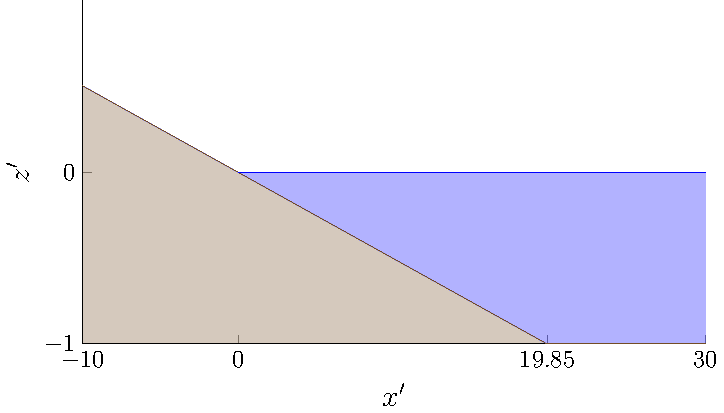
\includegraphics[width=\textwidth]{./Figures/Diagrams/WaveTankSynolakis/WavetankArtifical.pdf}
	\caption{Diagram showing a longitudinal section of the wave tank for the run-up experiment with the water (\squareF{blue}) and the bed (\squareF{brown!80!black}) where the coordinates have been non-dimensionalised \cite{Synolakis-1987-523}.}
	\label{fig:SynolakisWT}
\end{figure}

\begin{figure}
	\centering
	\begin{subfigure}{0.5\textwidth}
		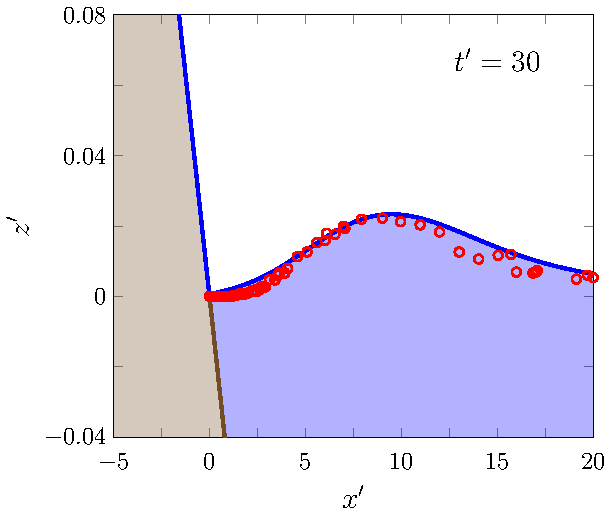
\includegraphics[width=\textwidth]{./Figures/Experimental/Synolakis/nonbreaking/30s.pdf}
		\vspace{0.5cm}
	\end{subfigure}%
	\begin{subfigure}{0.5\textwidth}
		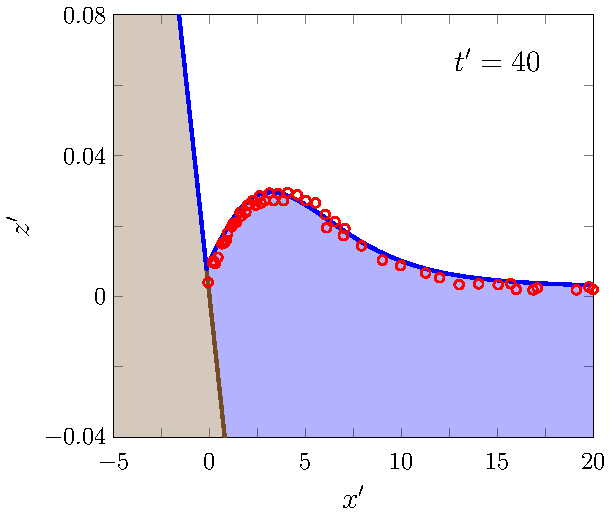
\includegraphics[width=\textwidth]{./Figures/Experimental/Synolakis/nonbreaking/40s.pdf}
		\vspace{0.5cm}
	\end{subfigure}
	\begin{subfigure}{0.5\textwidth}
		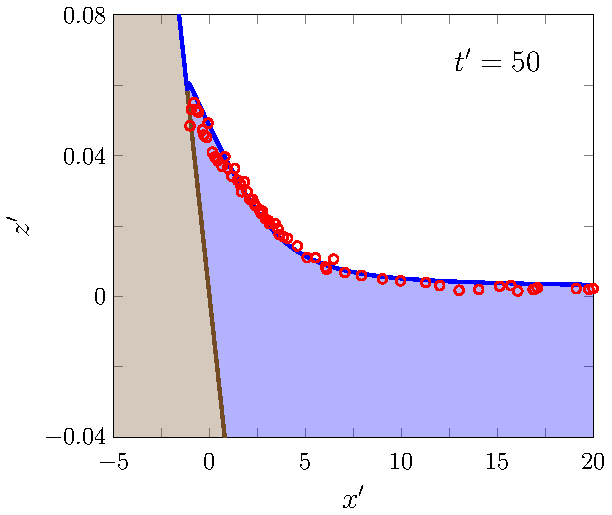
\includegraphics[width=\textwidth]{./Figures/Experimental/Synolakis/nonbreaking/50s.pdf}
		\vspace{0.5cm}
	\end{subfigure}%
	\begin{subfigure}{0.5\textwidth}
		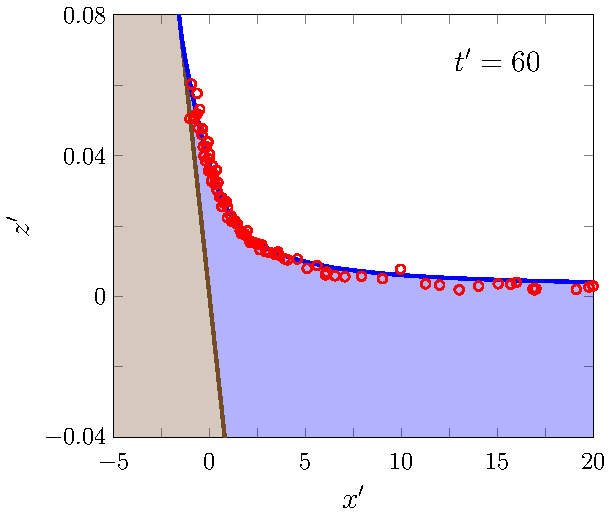
\includegraphics[width=\textwidth]{./Figures/Experimental/Synolakis/nonbreaking/60s.pdf}
		\vspace{0.5cm}
	\end{subfigure}
	\begin{subfigure}{0.5\textwidth}
		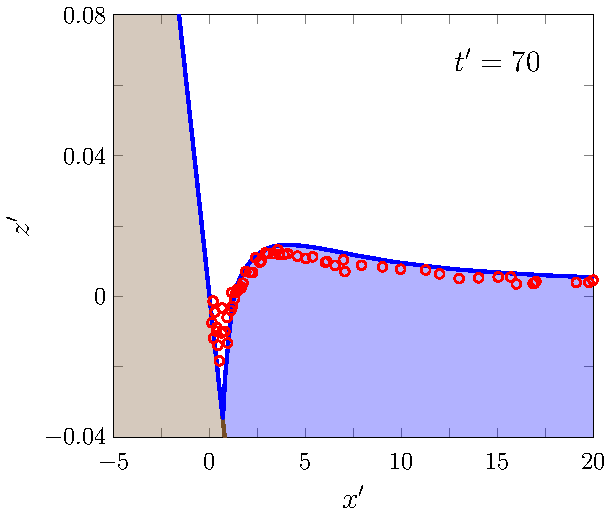
\includegraphics[width=\textwidth]{./Figures/Experimental/Synolakis/nonbreaking/70s.pdf}
		\vspace{0.5cm}
	\end{subfigure}
	\caption{A comparison of the water surface profiles $w'(x',t')$ for the experiment (\circlet{red}) and the numerical solution (\squareF{blue}) over the bed (\squareF{brown!60!black}) at various times.}
	\label{fig:SynolakisFEVMNoBreak}
\end{figure}

\begin{table}
	\centering
	\begin{tabular}{l  c  c c}
		Quantity& $\mathcal{C}^*\left(\vecn{q}^0\right)$ & $\mathcal{C}^*\left(\vecn{q}^*\right)$ & ${C}^*\left(\vecn{q}^0,\vecn{q}^*\right)$  \B\\
		\hline 
		$h'$ & $240.416965344$ & $240.416965376$ & $1.33\times 10^{-10}$ \T \\
		$u'h'$ & $-0.319050138516$ & $0.318891991793$ & $4.96\times 10^{-4}$\\
		$G'$ & $-0.319073723126$ & $0.318886191223$ & $5.88\times 10^{-4}$\\
		$\mathcal{H}'$ & $-118.389958187$ & $-118.3900028$ & $3.77 \times 10^{-7}$ \B\\
		\hline \\
	\end{tabular}
	\caption{Initial and final ($t'=200$) total amounts and the conservation error for the conserved quantities in the numerical solution of the run-up experiment. Here the absolute value of the total amount of $uh$ and $G$ are taken in the error as the wave is reflected off the beach.}
	\label{tab:ConservationSynFEVM}
\end{table}

\section{Comparison To Ritter's Dry-Bed Dam-Break Solution}

\end{document}